\documentclass[a4paper, 16pt]{article}
\usepackage[UTF8]{ctex}
\usepackage{geometry}
\usepackage{graphicx}
\usepackage{setspace}
\usepackage{float}
\usepackage{listings}
\usepackage{xcolor}
\lstset{
    numbers=left, 
    numberstyle= \tiny, 
    keywordstyle= \color{ blue!70},
    commentstyle= \color{red!50!green!50!blue!50}, 
    frame=shadowbox, % 阴影效果
    rulesepcolor= \color{ red!20!green!20!blue!20} ,
    escapeinside=``, % 英文分号中可写入中文
    xleftmargin=2em,xrightmargin=2em, aboveskip=1em,
    framexleftmargin=2em
} 
\geometry{left = 1.0 cm, right = 1.0cm, top = 2.0cm, bottom = 2.0cm	}
\title{编译原理第四章(一)}
\author{李鹏辉}

\begin{document}
\maketitle 
1. (4.2.1)考虑上下文无关文法 $S \rightarrow SS + | S S * | a$以及串$aa+a*$

1) 给出这个串的一个最左推导

$S \rightarrow SS* \rightarrow SS+S* \rightarrow aS+S* \rightarrow aa+S* \rightarrow aa+a*$\\

2)给出这个串的一个最右推导

$S \rightarrow SS* \rightarrow Sa* \rightarrow SS+a* \rightarrow Sa+a* \rightarrow aa+a* $\\

3)给出这个串的一颗语法分析树\\
\begin{figure}[H]
\centering
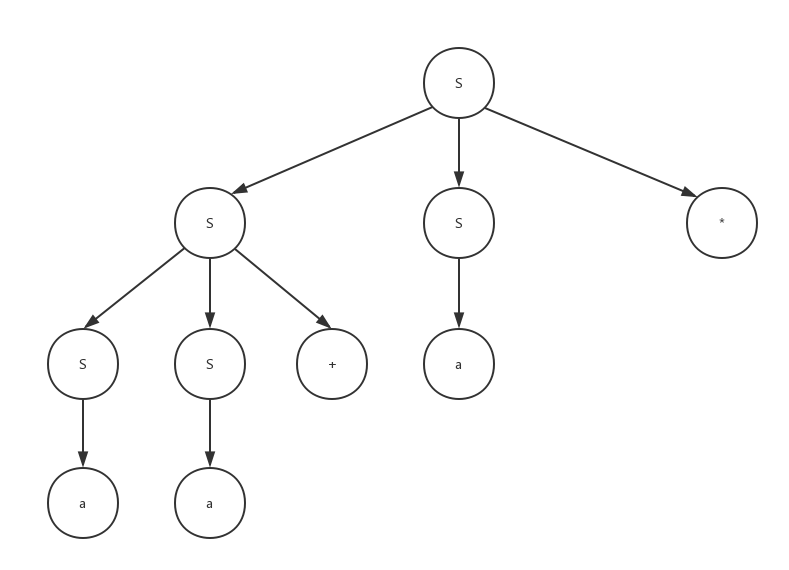
\includegraphics[scale = 0.4]{chapter4_hw1_1}
\caption{Parsing Tree}
\end{figure}

4)这个文法是否是二义性的? 证明你的回答(选作)

没有。

1)假设该文法存在二义性,则存在一个终结符串,使得能够根据该文法有两个或者多个语法分析树。

2) 根据文法定义, $S \rightarrow SS + | S S * | a$, $ S \rightarrow SS+$若存在二义性,则对于其右侧表达式,$SS+$中左$S$和右$S$至少有一个$S$存在二义性。同理$ S \rightarrow SS*$若存在二义性,则对于其右侧表达式,$SS+$中左$S$和右$S$至少有一个$S$存在二义性。

3)所以,取该终结符的两个不同的语法分析树,从根节点开始进行(跟-右-左)顺序遍历,并一一对比当前节点位置是否相同。

3).0 当前节点为S,进行比较。
	
		3).1 如果两棵树在当前节点之后的产生式都是运用$S \rightarrow a$,则回溯上一层节点,如果有左侧节点,则设置当前节点为其左侧S。跳到3).0执行
	
		3).2 如果两棵树在当前节点都是$S \rightarrow SS + $, 或者都是$ S\rightarrow S S *$则将当前节点设置成右侧S,跳到3).0执行。
	
		3).3 如果两棵树在当前节点推导形式不一致,则其中一个为$S \rightarrow a$,另外一个不是,则矛盾。因为$S \rightarrow a$将产生最右侧终结符a,而另一侧将产生+或者*. 同理,其中一个是$S \rightarrow SS + $, 另一个是$ S\rightarrow S S *$,最右侧终结符也不一致。 所以一旦改步骤运行到当前节点3).3,则两棵树产生的终结符串将会不一致,所以在此题设我的假设中,两棵树将不可能遍历到当前节点。只可能在上述其他节点。

4) 而其他节点表示每一层的推导运用的产生式均一致,则两棵树完全一致,和题设矛盾,所以该文法不存在二义性。\\

5)这个文法生成的语言是什么?

字母表为{a, +, *},运算对象为{a}的为加法和乘法的运算的后缀表达式。

2. 为(4.2.3)的第一题的语言设计文法:所有由0和1组成的并且每个0之后都至少跟着一个1的串的集合

$S \rightarrow A|BA$

$A \rightarrow \varepsilon|0B|AA$

$B \rightarrow \varepsilon|1B$\\

3. (4.3.1)下面是一个只包含符号a和b的正则表达式的文法,其中用+替代表示并运算的字符|,以避免和文法中作为元符号使用竖线混淆\\
\begin{table}[H]
\centering
\caption{Analysis}
\begin{tabular}{c}
\hline
$rexpr \rightarrow rexpr + rterm| rterm$\\
$rterm \rightarrow rterm \;rfactor | rfactor$\\
$rfactor \rightarrow rfactor* | rprimary$\\
$rprimary \rightarrow a | b$\\
\hline
\end{tabular}
\end{table}

1) 对该文法提取左公因子
\begin{table}[H]
\centering
\caption{Analysis}
\begin{tabular}{c}
\hline
$rexpr \rightarrow rexpr + rterm| rterm$\\
$rterm \rightarrow rterm \;rfactor | rfactor$\\
$rfactor \rightarrow rfactor* | rprimary$\\
$rprimary \rightarrow a | b$\\
\hline
\end{tabular}
\end{table}

2)提取左公因子的变换能是这个文法适用于自顶向下的语法分析技术吗?

不能,存在左递归。

3)将提取了左公因子的文法继续消除左递归


\begin{table}[H]
\centering
\caption{Analysis}
\begin{tabular}{c}
\hline
$rprimary \rightarrow a | b$ \\
$rfactor \rightarrow  rprimary \; rfactor'$\\
$rfactor' \rightarrow *rfactor'| \varepsilon$\\
$rterm \rightarrow rfactor \; rterm'$\\
$rterm' \rightarrow rfactor \; rterm' | \varepsilon$\\
$rexpr \rightarrow rterm \;  rexpr' $\\
$rexpr' \rightarrow +reterm \; rexpr' | \varepsilon$\\
\hline
\end{tabular}
\end{table}
4)此时得到的文法适用于自顶向下的语法分析吗?

适合,无左递归,满足条件。

\end{document}